\section{Introduction}
\subsection{Beamer Basics}

\begin{frame}[fragile] % fragile is needed whenever verbatim env. is called.
Welcome to \LaTeX\ beamer.\\~\
\begin{itemize}
    \item $\sum_{i=1}^m i^2=\dfrac{m(m+1)(2m+1)}{6}$\\~\
    \item \verb|$\sum_{i=1}^m i^2=\dfrac{m(m+1)(2m+1)}{6}$|
\end{itemize}
\end{frame}



\begin{frame}[fragile]{This is a Frame Title}
\begin{itemize}
    \item<1->Frames function as slides. All content must clearly be defined within a \verb+\begin{frame}+\ldots\verb+\end{frame}+ environment.
%\vspace{1em}
    \item<2-> Similar to frames, blocks are used to highlight important information via text, figures, formulae, equations, code, etc.
\end{itemize}
\begin{block}{Block name}<3->
This is a block. Similar to frames, all content within a block must be defined within a \verb+\begin{block}+\ldots\verb+\end{block}+.
\end{block}
\end{frame}

\subsection{Types of Blocks}
\begin{frame}[fragile]
\begin{enumerate}
    \item Here are two blocks in separate columns. Columns in beamer work differently compared to the \verb+multicols+ environment in other document classes.
    \begin{columns}
    \begin{column}{0.48\textwidth}
    \begin{block}{Column 1:}
    {\gray \lipsum[2][1-6]}
\\~\ % Used for spacing out the block 
    \end{block}
    \end{column}
    \begin{column}{0.48\textwidth}
    \begin{block}{Column 2:}
    {\gray \lipsum[1][1-6]}
\\~\ % Used for spacing out the block 
    \end{block}
    \end{column}
    \end{columns}
\end{enumerate}
\end{frame}

% \\~\ is used to force empty lines to generate to fix general typesetting within blocks.
% \\ = new line and ~\ = empty character (DO NOT CONFUSE FOR "\~")
% \lipsum is used to generate dummy text.

\begin{frame}
\begin{enumerate}
        \setcounter{enumi}{1}
        \item Here is an example of a lemma.
        \\
\begin{lemma}
\label{lemmaA}
    \alert{Lemma Name:} Body of Lemma.\\~\ 
    \\ Non-Numbered Equation:
    \begin{equation*}
    f = -X_1^2-X_2^2-\dots-X_\lambda^2+X_{\lambda+1}^2+\dots+X_m^2+c    
    \end{equation*}
    ~\\\ Numbered Equations:
    \begin{align}
    J(u):=&\int_\Omega \left( \frac{1}{2} \lvert \nabla u \rvert ^2 - F(u) \right)dx\\
    \begin{split}
        \Rightarrow\therefore J'(u)(v)=&\langle\nabla J(u),v\rangle =\int_\Omega\{(\nabla u\cdot\nabla v -f(u)v)\}dx, \\
        =&\int_\Omega(\Delta u -f(u))\cdot vdx,\qquad \forall v \in H 
    \end{split}
    \end{align}
\end{lemma}
\end{enumerate}
\end{frame}

\begin{frame}
\begin{enumerate}
\setcounter{enumi}{2}
\item Here is a definition block.

\begin{definition}[Term being defined]\label{definition}
{\gray \lipsum[3][1-7]}
\end{definition}

~\ % Shortcut to creating space without errors by creating a hidden character.

\item Here is a remark block.
\begin{remark}
Such blocks are suitable for \alert{pointing out or revising a fact}. You can recall elements as shown, Lemma~\ref{lemmaA}. Note the use of the $\sim$ character between words to prevent line-breaks.
\end{remark}
\end{enumerate}
\end{frame}

\begin{frame}
\begin{enumerate}
\setcounter{enumi}{4}
\item Here is an example of an example block.
\begin{example}
    Below is an example of a cited theorem. % You can customise your citation commands to specify the metadata of the document cited to show up in the footer of this slide instead.
\end{example}
\begin{theorem}[\textbf{Catalan-Mih\u{a}ilescu Theorem \cite{SMSB}}]
\label{CMT}
Let $p>q$ be prime numbers. Then the equation
\begin{equation}
    x^p -y^q = 1
\end{equation}
has no solutions in positive integers $x$ and $y$, other than $3^2 -2^3 = 1$.
\end{theorem}
\end{enumerate}
\end{frame}

\begin{frame}
\begin{enumerate}
\setcounter{enumi}{5}
\item Block environments such as {\yellow block}, {\red alertblock} and {\green exampleblock} can be used for creating other elements like so.
\begin{alertblock}{Notation}
    We denote the set of continuously differentiable functions within the domain $[a,b]$ as $C^1[a,b]$.
\end{alertblock}
\begin{exampleblock}{Special Case 1:}
    The most notable exception to the general rule that uncountable sets must have non-zero measures is the \alert{Cantor set}, which consists of iteratively deleting the open middle third of an interval, say, $[0,1]$.
    \\~\\\
    Hence, the measure of the removed interval length:
    \begin{equation}\label{specialcase}
        m\left([0,1]-\mathcal{C}_{[0,1]}\right)=\sum_{n=0}^\infty\frac{2^n}{3^{n+1}}
        =\frac{1}{3}\left(\frac{1}{1-\frac{2}{3}}\right)=1\tag{SC1}
    \end{equation}
    \[\Rightarrow m\left(\mathcal{C}_{[0,1]}\right)=0\]
    $\therefore$ by \eqref{specialcase}, the measure of our Cantor set is zero.
\end{exampleblock}
\end{enumerate}    
\end{frame}

\subsection{Overlays for Uncovering Lists Piecewise/Itemwise}

\begin{frame}
    Here is an example of a list being uncovered piecewise.
\begin{enumerate}
    \item<1-> Item 1 comes first.
    \item<2-> Item 2 comes second.
    \item<3-> Item 3a and
    \item<3-> Item 3b both appear at the same time.
\end{enumerate}
\begin{remark}<4->
    Blocks and other objects can be uncovered as well.
\end{remark}
\end{frame}


\subsection{Proofs Blocks over Proof Block}
{ \renewcommand{\proofname}{Long Proof} % Used to rename \proofname from its default value, `proof'
\begin{frame}
We used the custom-defined block `\textbf{proofs}' instead of `\textbf{proof}' when our proof exceeds one slide as this allows us to chain it as shown.
\\~\


    \begin{proofs}
    \begin{enumerate}
        \item  {\gray \lipsum[6][1-6]}
    \end{enumerate}
    \end{proofs}
    \end{frame}
    
    \begin{frame}
    \begin{columns}
        \begin{column}{0.48\textwidth}
            \begin{proofs}[\proofname\ (Cont.)]
            \begin{enumerate}
            \setcounter{enumi}{1}
            \item {\gray \lipsum[6][7-11]}
            \end{enumerate}
            \end{proofs}
        \end{column}
        \begin{column}{0.48\textwidth}
            \begin{figure}
            \centering
            % 3D Cone
% Author: Gene Ressler. Adapted to TikZ by Kjell Magne Fauske.
% See http://www.frontiernet.net/~eugene.ressler/ for more details.

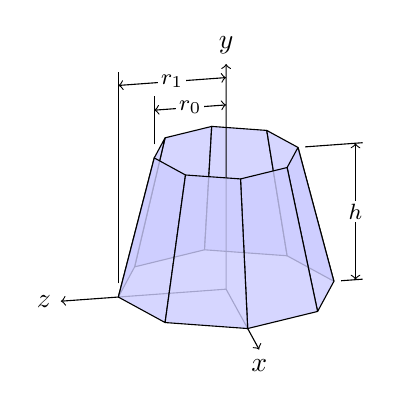
\begin{tikzpicture}[join=round]
    \tikzstyle{conefill} = [fill=blue!20,fill opacity=0.8]
    \tikzstyle{ann} = [fill=white,font=\footnotesize,inner sep=1pt]
    \tikzstyle{ghostfill} = [fill=white]
         \tikzstyle{ghostdraw} = [draw=black!50]
    \filldraw[conefill](-.775,1.922)--(-1.162,.283)--(-.274,.5)
                        --(-.183,2.067)--cycle;
    \filldraw[conefill](-.183,2.067)--(-.274,.5)--(.775,.424)
                        --(.516,2.016)--cycle;
    \filldraw[conefill](.516,2.016)--(.775,.424)--(1.369,.1)
                        --(.913,1.8)--cycle;
    \filldraw[conefill](-.913,1.667)--(-1.369,-.1)--(-1.162,.283)
                        --(-.775,1.922)--cycle;
    \draw(1.461,.107)--(1.734,.127);
    \draw[arrows=<->](1.643,1.853)--(1.643,.12);
    \filldraw[conefill](.913,1.8)--(1.369,.1)--(1.162,-.283)
                        --(.775,1.545)--cycle;
    \draw[arrows=->,line width=.4pt](.274,-.5)--(0,0)--(0,2.86);
    \draw[arrows=-,line width=.4pt](0,0)--(-1.369,-.1);
    \draw[arrows=->,line width=.4pt](-1.369,-.1)--(-2.1,-.153);
    \filldraw[conefill](-.516,1.45)--(-.775,-.424)--(-1.369,-.1)
                        --(-.913,1.667)--cycle;
    \draw(-1.369,.073)--(-1.369,2.76);
    \draw(1.004,1.807)--(1.734,1.86);
    \filldraw[conefill](.775,1.545)--(1.162,-.283)--(.274,-.5)
                        --(.183,1.4)--cycle;
    \draw[arrows=<->](0,2.34)--(-.913,2.273);
    \draw(-.913,1.84)--(-.913,2.447);
    \draw[arrows=<->](0,2.687)--(-1.369,2.587);
    \filldraw[conefill](.183,1.4)--(.274,-.5)--(-.775,-.424)
                        --(-.516,1.45)--cycle;
    \draw[arrows=<-,line width=.4pt](.42,-.767)--(.274,-.5);
    \node[ann] at (-.456,2.307) {$r_0$};
    \node[ann] at (-.685,2.637) {$r_1$};
    \node[ann] at (1.643,.987) {$h$};
    \path (.42,-.767) node[below] {$x$}
        (0,2.86) node[above] {$y$}
        (-2.1,-.153) node[left] {$z$};
\end{tikzpicture}
            \caption{3D Cone designed by Gene R., see \texttt{Images/Figures/3D\_Cone.tex}}
            \end{figure}
        \end{column}
    \end{columns}
    \end{frame}
    
    \begin{frame}[fragile=singleslide]
    The `proofs' blocks also allow us to throw in text in between blocks like so\dots 
    \begin{remark}
    \ldots as well as remarks, definitions and so on.
    \end{remark}
    
    \begin{proofs}[\proofname\ (Cont.)]
    \begin{enumerate}
    \setcounter{enumi}{2}
    \item Remember, discontinuous lists and piece-wise overlays work here as well. 
    \\~\ \\
    {\gray \lipsum[5][2-4]} \qed
    \end{enumerate}~\
    \end{proofs}
    \begin{remark}
    End your \verb+proofs+ block with the `\verb+\qed+' command to signify the end of the proof.
    \end{remark}
    \end{frame}
}

\begin{frame}
    Another helpful feature is the inclusion of appendices, which allow you to add supplementary slides to your presentation. This is especially useful when you want to keep ready any prerequisite data or case studies that may fall outside the immediate scope of the presentation topic. 
    \\~\ \\ An example of the use of an appendix\dotfill (\hyperlink{app1}{A1})\quad or\quad\hyperlink{app1}{\beamergotobutton{Appendix I}}
    \\~\ \\
    This does not contribute to the total slides displayed in the top left corner; the appendix and reference slides are accounted for separately at the end.
\end{frame}